\documentclass[]{book}
\usepackage{lmodern}
\usepackage{amssymb,amsmath}
\usepackage{ifxetex,ifluatex}
\usepackage{fixltx2e} % provides \textsubscript
\ifnum 0\ifxetex 1\fi\ifluatex 1\fi=0 % if pdftex
  \usepackage[T1]{fontenc}
  \usepackage[utf8]{inputenc}
\else % if luatex or xelatex
  \ifxetex
    \usepackage{mathspec}
  \else
    \usepackage{fontspec}
  \fi
  \defaultfontfeatures{Ligatures=TeX,Scale=MatchLowercase}
\fi
% use upquote if available, for straight quotes in verbatim environments
\IfFileExists{upquote.sty}{\usepackage{upquote}}{}
% use microtype if available
\IfFileExists{microtype.sty}{%
\usepackage[]{microtype}
\UseMicrotypeSet[protrusion]{basicmath} % disable protrusion for tt fonts
}{}
\PassOptionsToPackage{hyphens}{url} % url is loaded by hyperref
\usepackage[unicode=true]{hyperref}
\hypersetup{
            pdftitle={ICT Gender-Equality Paradox},
            pdfauthor={Mandy Davis},
            pdfborder={0 0 0},
            breaklinks=true}
\urlstyle{same}  % don't use monospace font for urls
\usepackage{natbib}
\bibliographystyle{plainnat}
\usepackage{longtable,booktabs}
% Fix footnotes in tables (requires footnote package)
\IfFileExists{footnote.sty}{\usepackage{footnote}\makesavenoteenv{long table}}{}
\usepackage{graphicx,grffile}
\makeatletter
\def\maxwidth{\ifdim\Gin@nat@width>\linewidth\linewidth\else\Gin@nat@width\fi}
\def\maxheight{\ifdim\Gin@nat@height>\textheight\textheight\else\Gin@nat@height\fi}
\makeatother
% Scale images if necessary, so that they will not overflow the page
% margins by default, and it is still possible to overwrite the defaults
% using explicit options in \includegraphics[width, height, ...]{}
\setkeys{Gin}{width=\maxwidth,height=\maxheight,keepaspectratio}
\IfFileExists{parskip.sty}{%
\usepackage{parskip}
}{% else
\setlength{\parindent}{0pt}
\setlength{\parskip}{6pt plus 2pt minus 1pt}
}
\setlength{\emergencystretch}{3em}  % prevent overfull lines
\providecommand{\tightlist}{%
  \setlength{\itemsep}{0pt}\setlength{\parskip}{0pt}}
\setcounter{secnumdepth}{5}
% Redefines (sub)paragraphs to behave more like sections
\ifx\paragraph\undefined\else
\let\oldparagraph\paragraph
\renewcommand{\paragraph}[1]{\oldparagraph{#1}\mbox{}}
\fi
\ifx\subparagraph\undefined\else
\let\oldsubparagraph\subparagraph
\renewcommand{\subparagraph}[1]{\oldsubparagraph{#1}\mbox{}}
\fi

% set default figure placement to htbp
\makeatletter
\def\fps@figure{htbp}
\makeatother

\usepackage{booktabs}
\usepackage{amsthm}
\makeatletter
\def\thm@space@setup{%
  \thm@preskip=8pt plus 2pt minus 4pt
  \thm@postskip=\thm@preskip
}
\makeatother

\title{ICT Gender-Equality Paradox}
\author{Mandy Davis}
\date{2020-10-08}

\begin{document}
\maketitle

{
\setcounter{tocdepth}{1}
\tableofcontents
}
\chapter{Exploratory Data Analysis}\label{exploratory-data-analysis}

\section{The Paradox}\label{the-paradox}

Gender equality (as measured by the Global Gender Gap Index) is
moderately, negatively correlated with the percentage of women among
ICT, adjusted for equal graduation numbers of men and women
(\(r = -0.47\), \(p < 0.001\)).

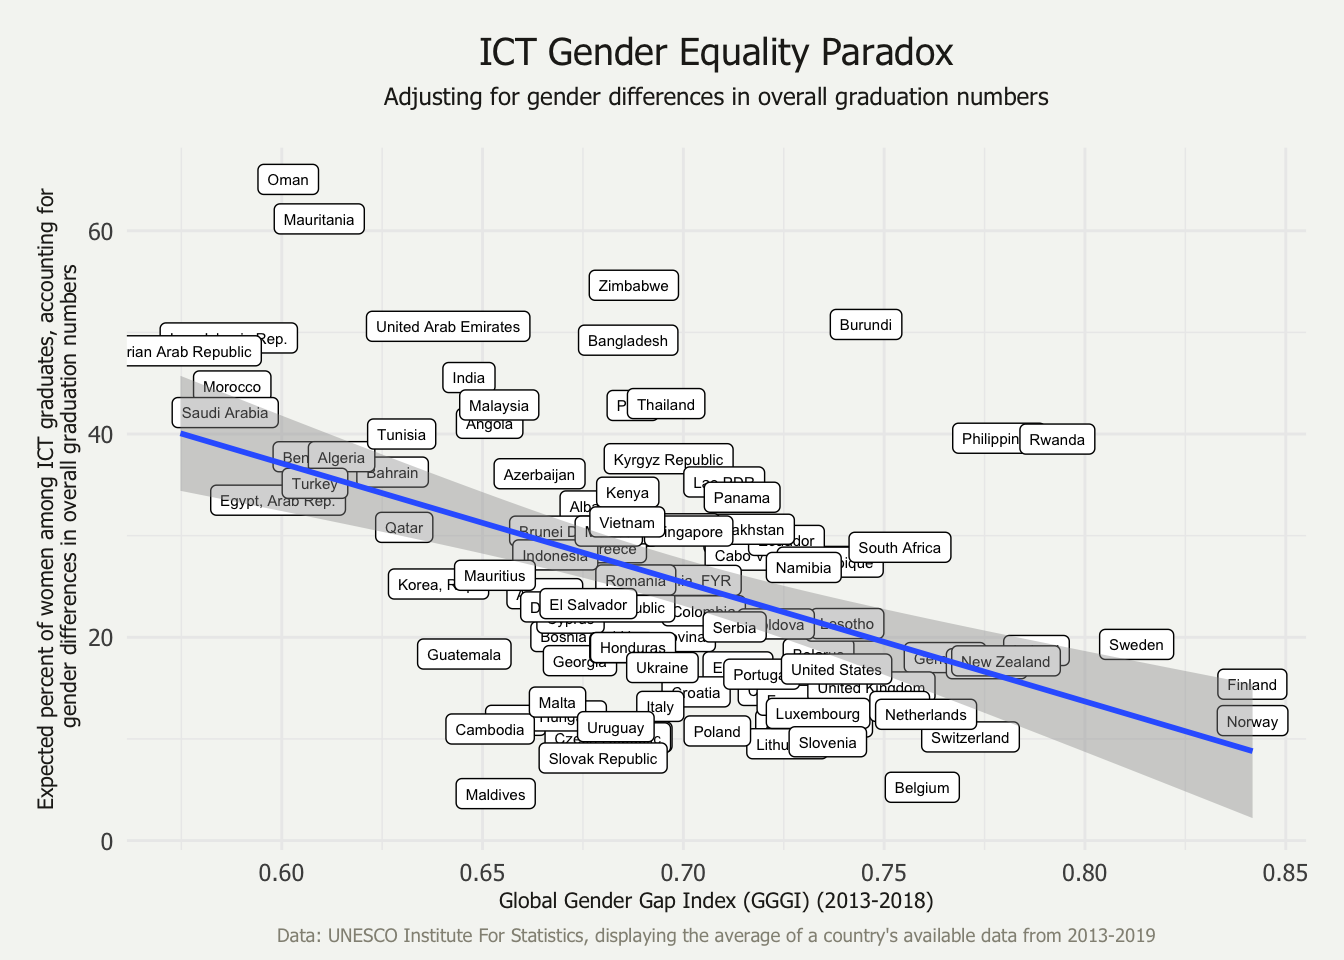
\includegraphics{bookdown-demo_files/figure-latex/paradox-1.pdf}

\section{ICT Graduation Rates in 7
Countries}\label{ict-graduation-rates-in-7-countries}

\textbf{{[}in progress{]}} I am working on creating the visualization
for all seven countries so that I can stack them and demonstrate the
disconnect there can be between the overall ratio of men and women
graduates and the \emph{percentage of all men and all women} who pursue
ICT.

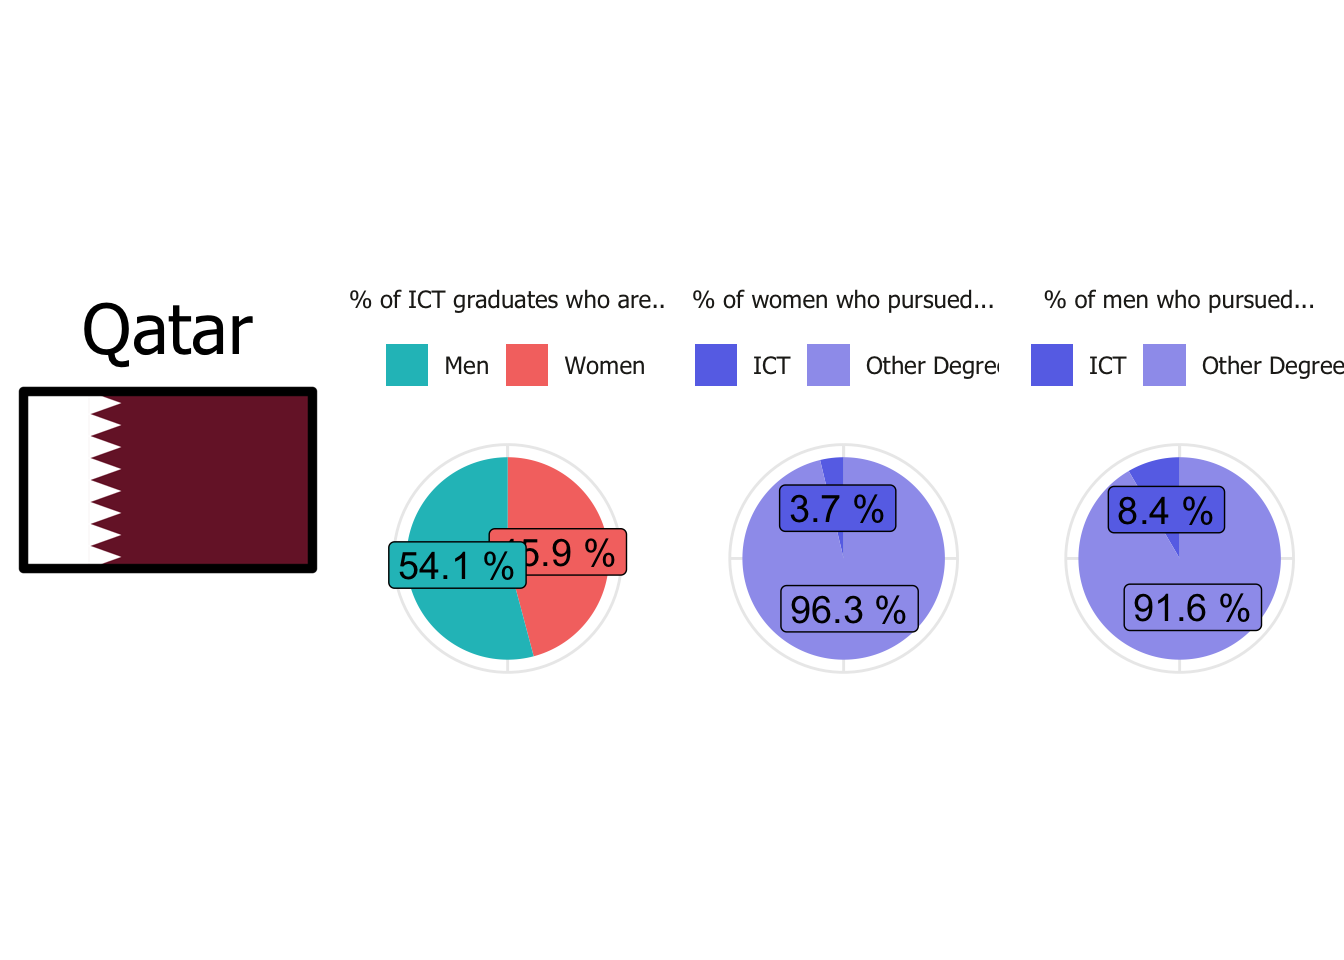
\includegraphics{bookdown-demo_files/figure-latex/flagtest-1.pdf}

\section{ICT Graduation Trends (Change Over
Time)}\label{ict-graduation-trends-change-over-time}

Less data than I would prefer, but that's helpful info too!

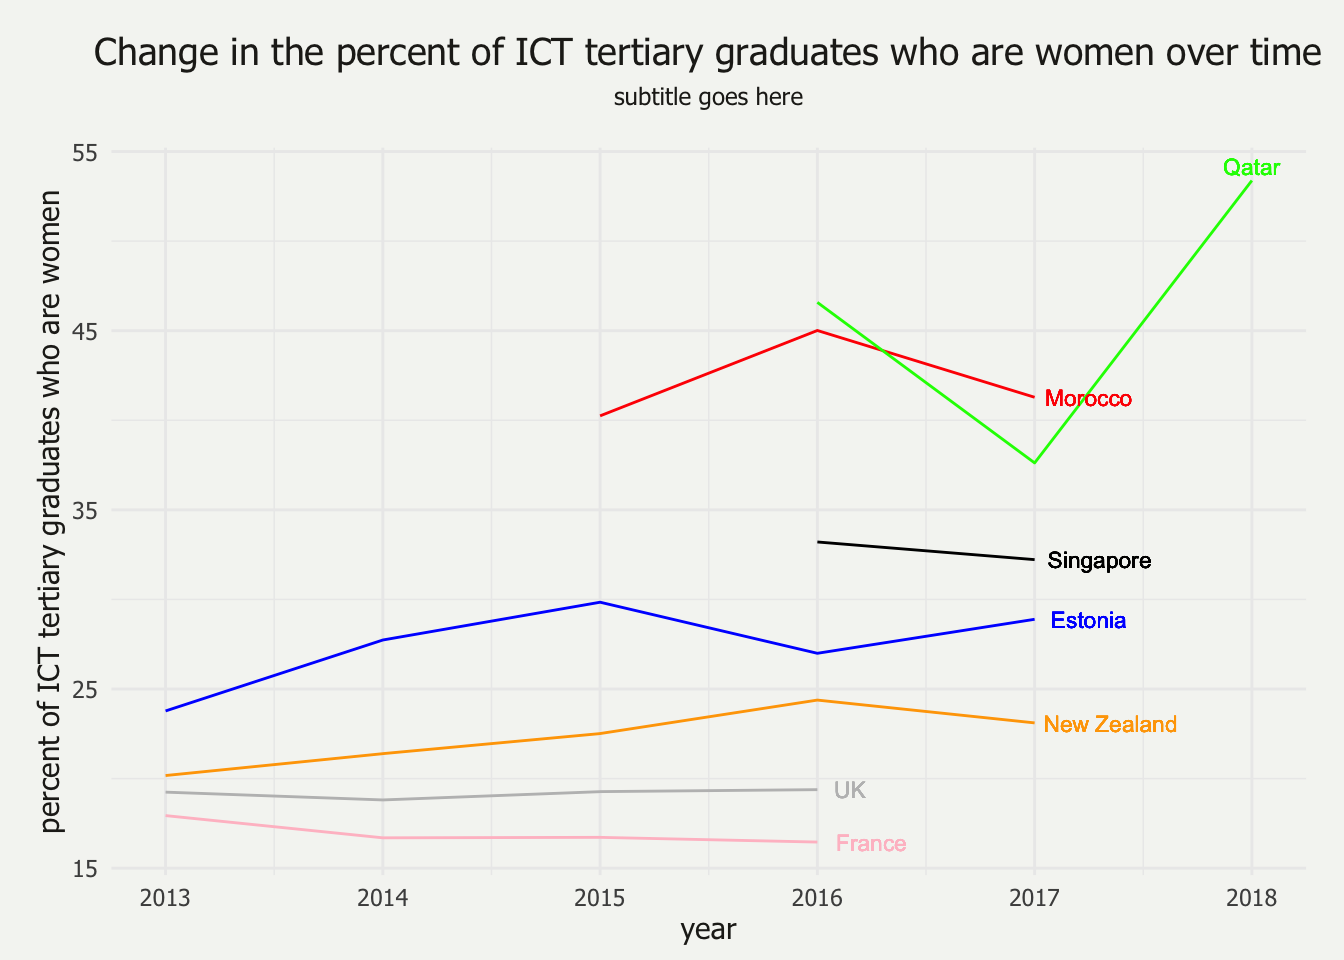
\includegraphics{bookdown-demo_files/figure-latex/ICT_change-1.pdf}

\section{Internet Usage}\label{internet-usage}

This is another reason I am so interested in comparing Qatar and
Morocco.

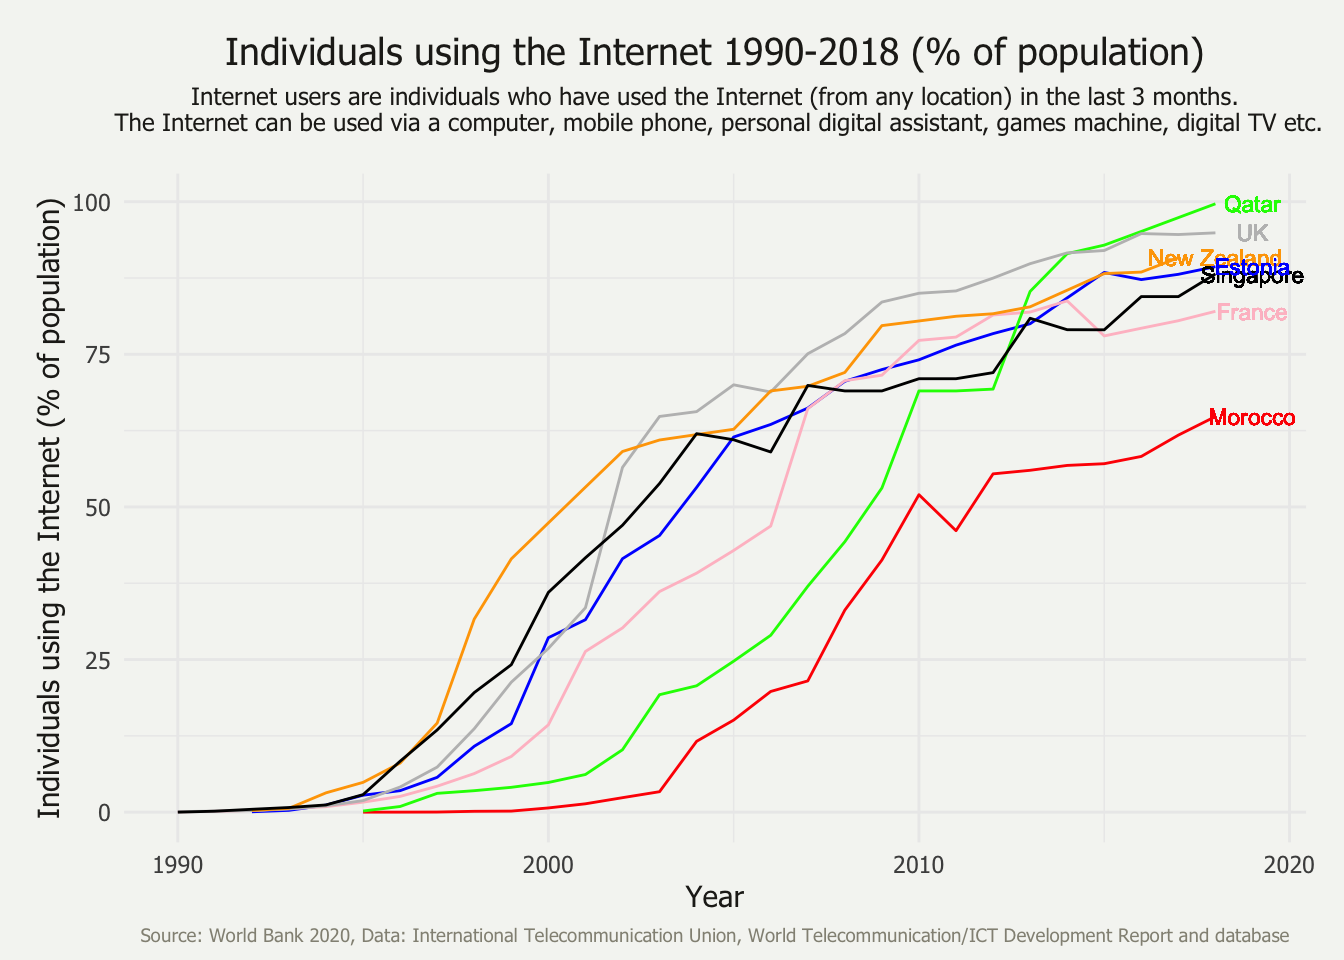
\includegraphics{bookdown-demo_files/figure-latex/internet-1.pdf}

\section{Interest: Oregon Vocational Interest Scales (ORVIS) from the
SAPA
Project}\label{interest-oregon-vocational-interest-scales-orvis-from-the-sapa-project}

A common argument for why the STEM and ICT Gender-Equality paradoxes
might exist surrounds the level of interest women have in the subjects.
In countries with a high level of gender equality, some argue, women are
free to pursue what they truly are interested in, even if those fields
are less lucrative.

In their controversial paper, Stoet \& Geary examined this using the
Programme for International Student Assessment (PISA) dataset. Interest
is also important because of its relationship with achievement. The PISA
data is valuable for understanding the interests of 15-year-olds who
live in OECD countries, however, it lack insight on the interests of
adults.

The Synthetic Aperture Personality Assessment (SAPA) collects data that
can fill that gap. SAPA is an online survey created by Northwestern
psychologist William Revelle that anyone with access to a web browser
and internet connection can take (\url{https://www.sapa-project.org/}).
The Oregon Vocational Interest Scales (ORVIS) are a component of SAPA.

The ORVIS contains seven total scales: Leadership, Organization,
Altruism, Creativity, Analysis, Production, Adventure, and Erudation.
The Analysis scale is the scale of interest for this research. Ten items
compose this scale, all of which are positively scored. The items are as
follows:

\begin{itemize}
\tightlist
\item
  Be a chemist
\item
  Design a laboratory experiment
\item
  Be a mathematician
\item
  Explain scientific concepts to others
\item
  Be a physicist
\item
  Carry out medical research
\item
  Be a scientific reporter
\item
  Solve complex puzzles
\item
  Develop a computer program
\item
  Be a statistician
\end{itemize}

Of the people who took the SAPA test from August 18, 2010 through
February 7, 2017, 219,728 indicated they are from a country that ended
up having 500 or more subjects during that time period. These people
form the final dataset used for analysis. Participants choose between
``male'' and ``female'' to select their gender identity, with
\(63.52\%\) (\(N = 139,567\)) identifying as female and the other
\(36.48\%\) (\(N = 80,162\)) identifying as male. The median age of the
particpants is 22, ranging from 14 to 90.

Below is a visualization of how these participants scored on their level
of analytical interest.

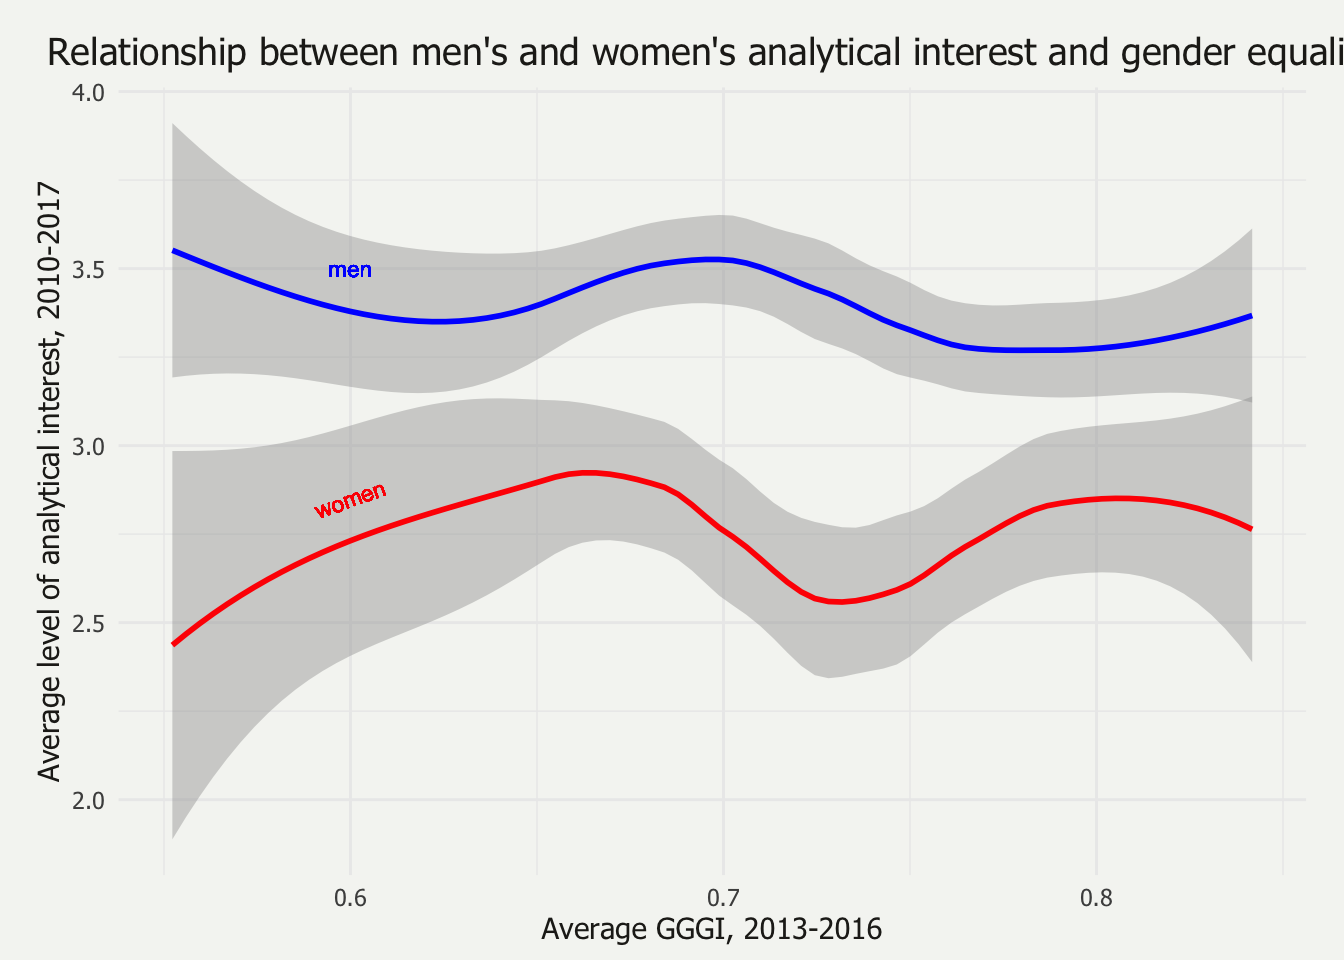
\includegraphics{bookdown-demo_files/figure-latex/orvis_both-1.pdf}

Next up is the same graph, but only for women's interest and with
country names included for reference.

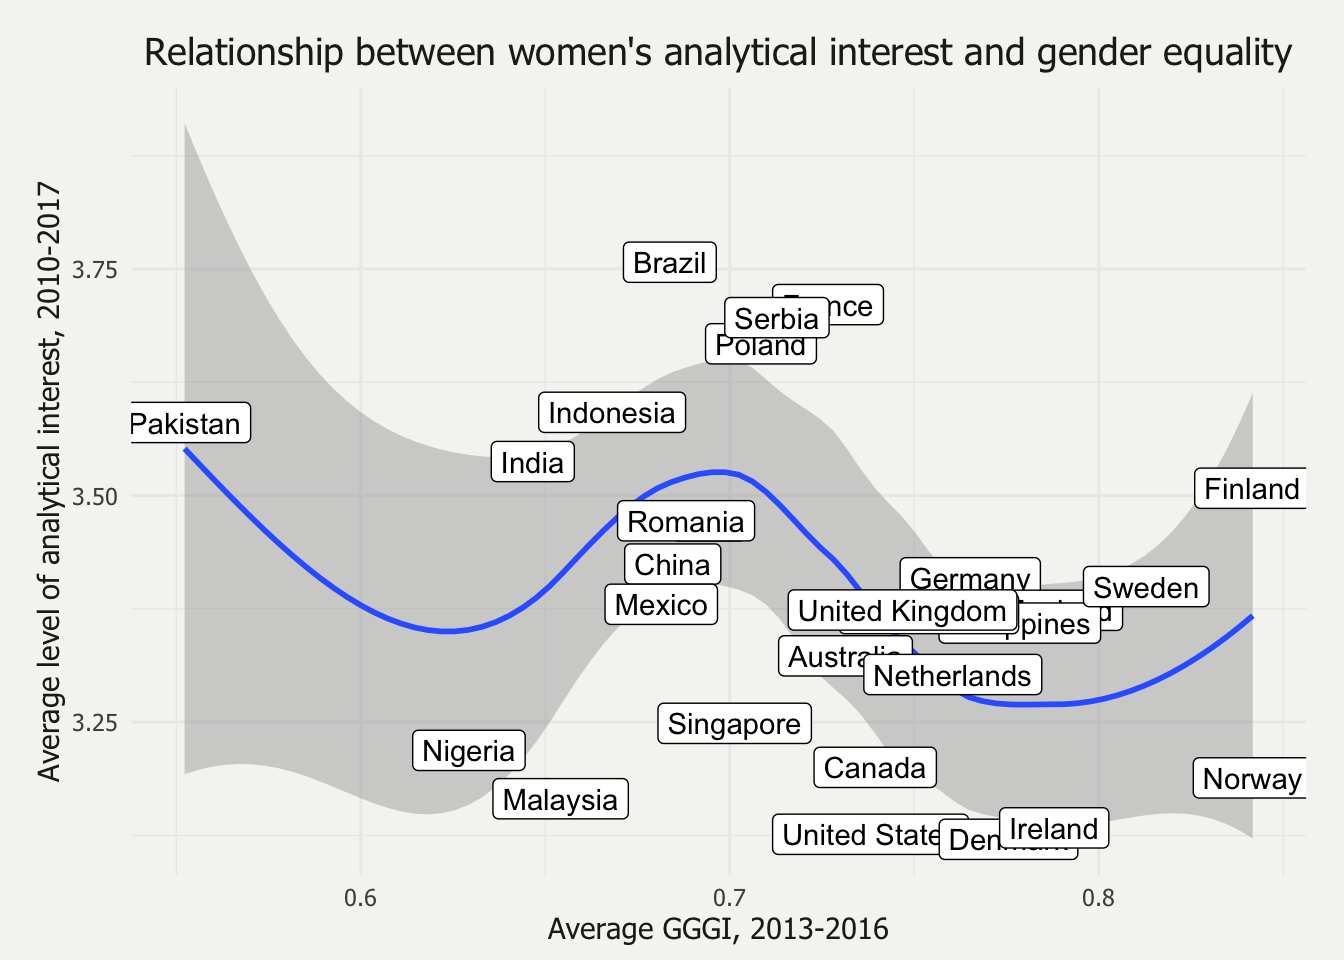
\includegraphics{bookdown-demo_files/figure-latex/interest_country-1.pdf}

\textbf{What does this mean?} I don't know (yet). There seems to be no
clear correlation like that of the ICT-GEP. However, it almost appears
that men's and women's interest are inversely proportional, which is a
really interesting lead, as men's and women's interest are theoretically
independent and have no cap. Contrast this to the proportion of men and
women there are in a given classroom---the proportions are dependent
upon one another, so we would expect this relationship. In this
situation, however, a relationship like this is not expected (without
considering the broader context).

\chapter{Mapping the ICT-GEP}\label{maps}

Before diving into the data, these maps offer a visual explanation of
the ICT-GEP when using the analysis method from the UNESCO think piece.

\section{Percent of women among ICT Graduates
worldwide}\label{percent-of-women-among-ict-graduates-worldwide}

\begin{center}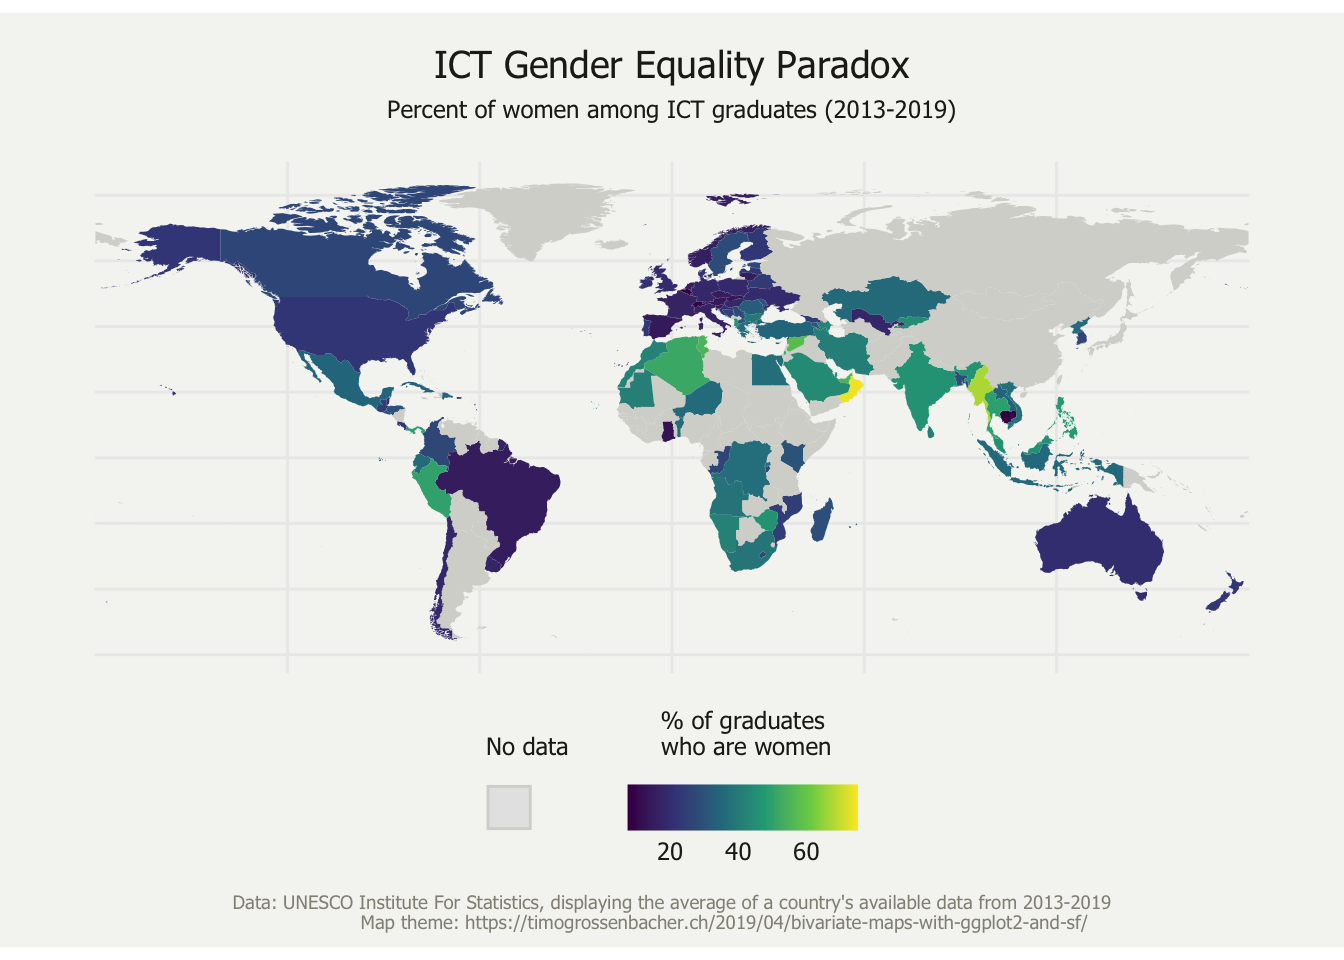
\includegraphics{bookdown-demo_files/figure-latex/ict_map-1} \end{center}

Note the visual reversal of colors when comparing the ICT map to the
GGGI map. This is exactly the idea behind the ICT-GEP: the higher the
gender equality, the lower the percentage of women among ICT graduates.

\section{Global Gender Gap Index
worldwide}\label{global-gender-gap-index-worldwide}

\begin{center}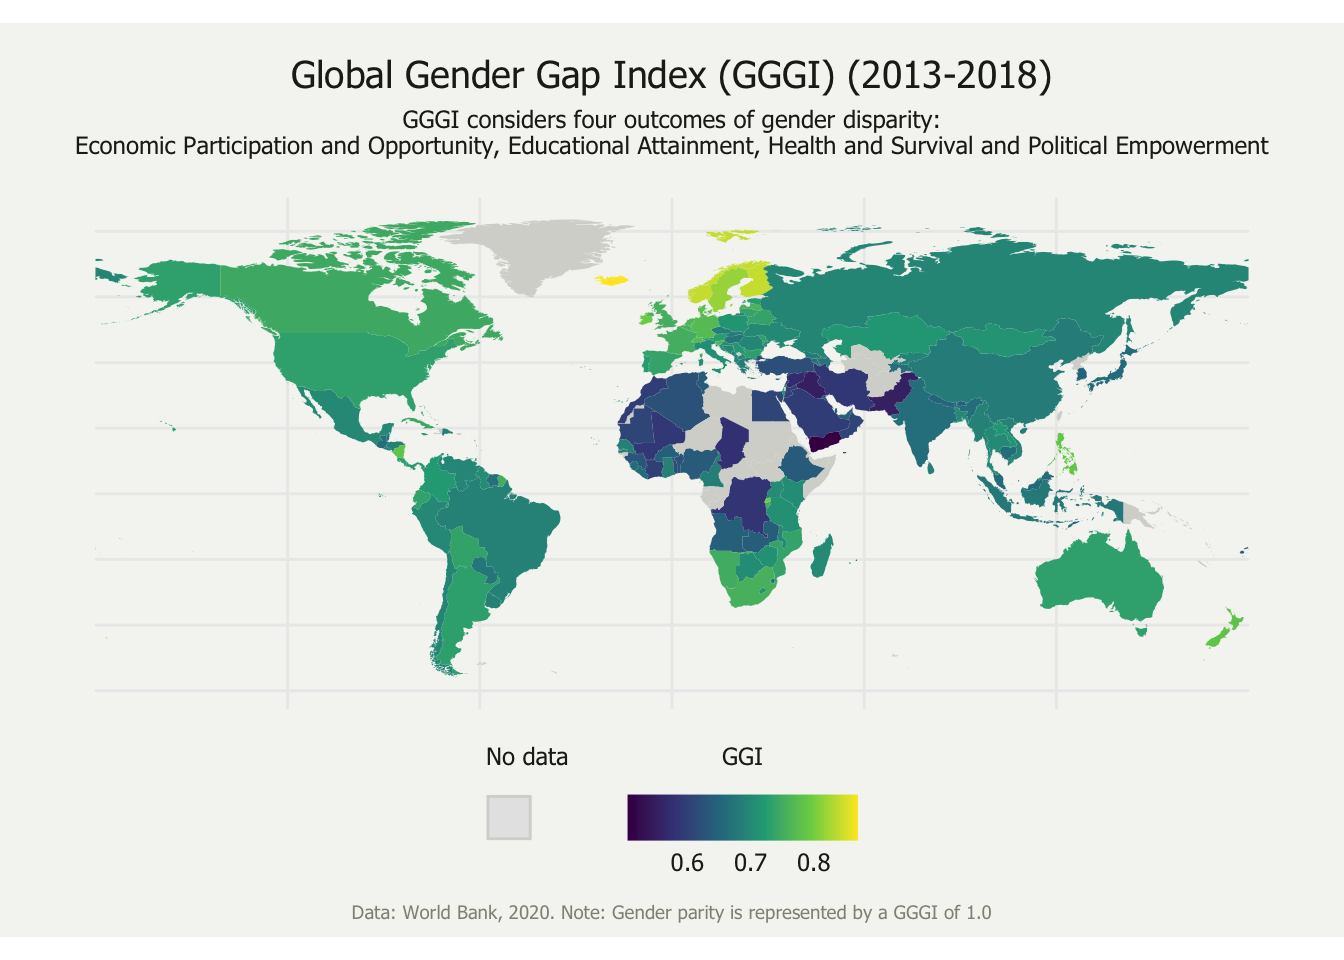
\includegraphics{bookdown-demo_files/figure-latex/ggi_map-1} \end{center}

\bibliography{ict-gep.bib}

\end{document}
